%%%%%%%%%%%%%%%%%%%%%%%%%%%%%%%%%%%%%%%%%%%%%%%%%%%%%%%%%%%%%%%%%%%%%%%%%%%
% Copyright (c) 2010 committers of YAKINDU and others.
% All rights reserved. This program and the accompanying materials
% are made available under the terms of the Eclipse Public License v1.0
% which accompanies this distribution, and is available at
% http://www.eclipse.org/legal/epl-v10.html
%
% Contributors:
%     committers of YAKINDU - initial API and implementation
%%%%%%%%%%%%%%%%%%%%%%%%%%%%%%%%%%%%%%%%%%%%%%%%%%%%%%%%%%%%%%%%%%%%%%%%%%%
\section{Generating Source Code}

\subsection{Create Xtend Project}
The starting point to create Java source code from a YAKINDU Statechart model
is to set up a Java project to contain the generated code. For the sake of
simplicity, we will instead create a new Xtend project for this purpose (Xtend
projects also possess the Java as well as the PDE Plugin project nature), as
this allows to easily manage dependencies and execute MWE workflows. As
outlined by Figures \ref{fig:screenshot4}, \ref{fig:screenshot5}, and
\ref{fig:screenshot6}, creating an Xtend project is easily done using the
respective project creation wizard. Here, we choose \emph{TrafficLightJavaDemo}
as the name of the project.

\begin{figure}[h!]
\center
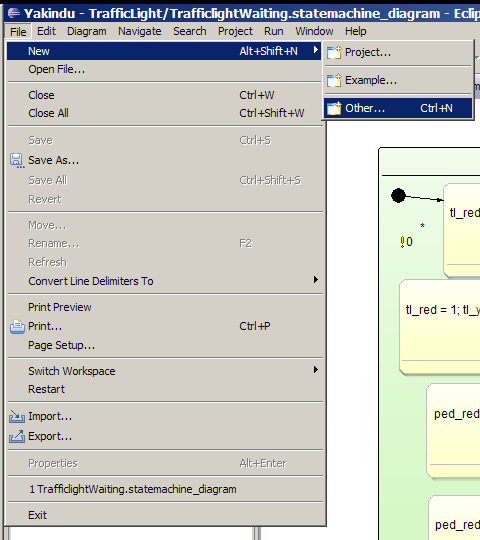
\includegraphics[width=0.5\textwidth]{./Pictures/Screenshot4}
\caption{\label{fig:screenshot4} Open New Wizard}
\end{figure}

\begin{figure}[h!]
\center
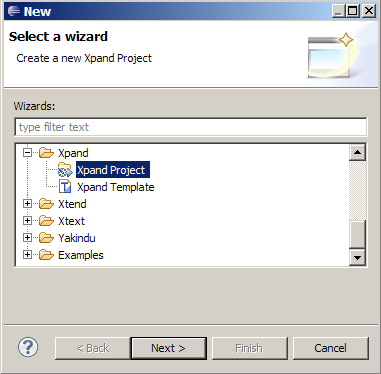
\includegraphics[width=0.5\textwidth]{./Pictures/Screenshot5}
\caption{\label{fig:screenshot5} Selecting to Create a new Xpand Project}
\end{figure}

\begin{figure}[h!]
\center
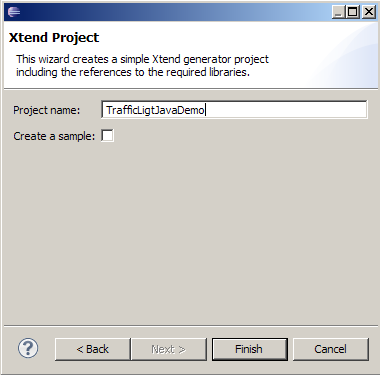
\includegraphics[width=0.5\textwidth]{./Pictures/Screenshot6}
\caption{\label{fig:screenshot6} Xtend Project Creation Wizard}
\end{figure}

%\begin{figure}[h!]
%\center
%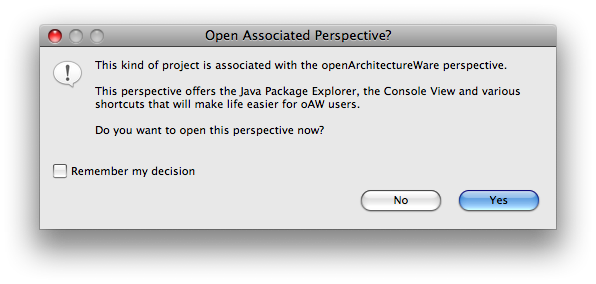
\includegraphics[width=0.8\textwidth]{./Pictures/Screenshot7}
%\caption{\label{fig:screenshot7}}
%\end{figure}
\clearpage
\subsection{Manage Dependencies}
Having created the \emph{TrafficLightJavaDemo} project by means of the Xtend
project wizard, the next step is to make the YAKINDU Java code generator plugin
visible within the local project's classpath, so the Java code generation
cartridge file, which is deployed by the code generator plugin, can be
referenced from a local MWE workflow (to be set up as the next step). As we
have created a Xpand project (which is implicitly also a PDE plugin project, as
the Xpand project wizard adds the PDE plugin project nature to it), we may simply
do so by adding the YAKINDU Statchart Java code generator plugin to the list of
dependent plugins of our local project. As outlined by Figures
\ref{fig:screenshot8} and \ref{fig:screenshot9}, this can be simply achieved by
opening the manifest editor on the \texttt{MANIFEST.MF} file located within the
\texttt{META-INF} folder of the project, selecting the \texttt{Dependencies}
tab (depicted by Figure \ref{fig:screenshot8}, then by choosing to \emph{Add} a
new dependency and selecting the YAKINDU Statechart Java code generator
plugin in the resulting dialog (depicted Figure \ref{fig:screenshot9}).
Also the following Plug-Ins are required:
\begin{itemize}
\item org.eclipse.jface.text
\item org.eclipse.emf.mwe.utils
\item org.eclipse.emf.ecore.xmi
\item org.antlr.runtime
\item org.eclipse.xtext
\item org.eclipse.xtext.log4j
\item com.ibm.icu
\item org.eclipse.core.runtime
\item org.eclipse.jdt.core
\end{itemize}

\begin{figure}[h!]
\center
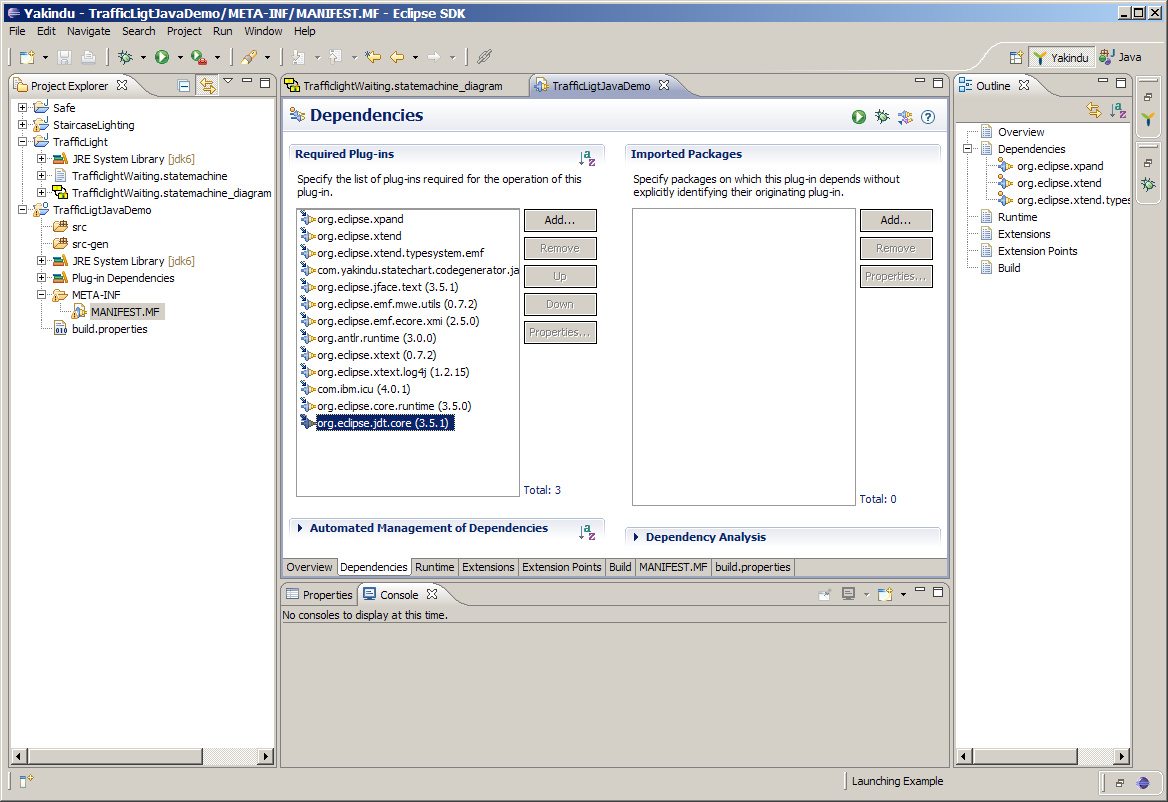
\includegraphics[width=\textwidth]{./Pictures/Screenshot8}
\caption{\label{fig:screenshot8} Manifest Editor}
\end{figure}

\begin{figure}[h!]
\center
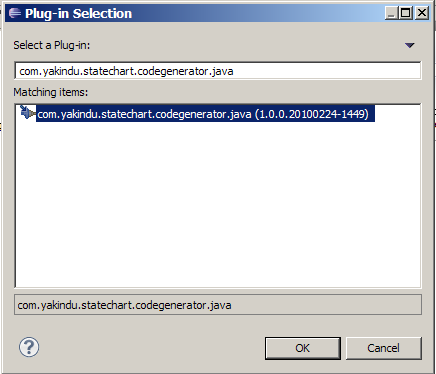
\includegraphics[width=0.5\textwidth]{./Pictures/Screenshot9}
\caption{\label{fig:screenshot9} Adding Plugin Dependency}
\end{figure}

\clearpage
\subsection{Create MWE Workflow File}
As the YAKINDU Java code generator plugin provides an OAW workflow cartridge
that may most simply be called from within a local MWE workflow file, the next
step is to now set up such an MWE workflow file. This can be done as depicted
by Figures \ref{fig:screenshot10}, \ref{fig:screenshot11}, and
\ref{fig:screenshot12}, choosing \texttt{generate.wme} as the name of the
workflow file.

\begin{figure}[h!]
\center
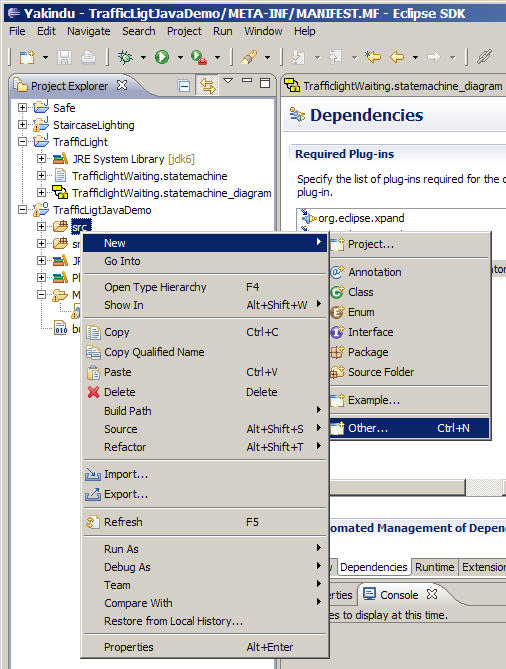
\includegraphics[width=0.5\textwidth]{./Pictures/Screenshot10}
\caption{\label{fig:screenshot10} Opening New File Creation Wizard}
\end{figure}

\begin{figure}[h!]
\center
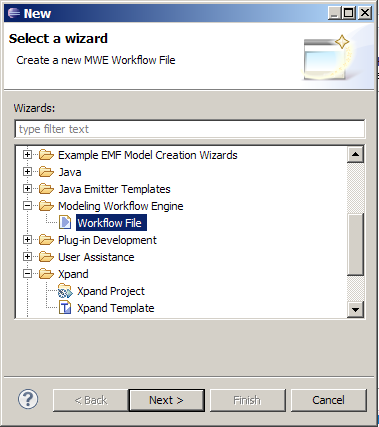
\includegraphics[width=0.5\textwidth]{./Pictures/Screenshot11}
\caption{\label{fig:screenshot11} Selecting to Create a new MWE Workflow File}
\end{figure}

\begin{figure}[h!]
\center
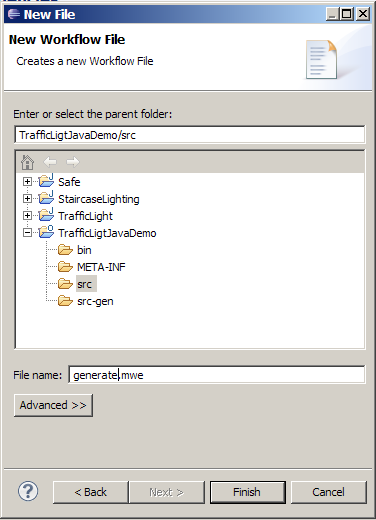
\includegraphics[width=0.5\textwidth]{./Pictures/Screenshot12}
\caption{\label{fig:screenshot12} Specifying Name of MWE Workflow File}
\end{figure}

\clearpage
The contents of the workflow file has to be added as outlined by
\ref{fig:screenshot13}. Basically, the location of the input YAKINDU
Statechart model (property \texttt{model}), as well as that of the output
folder (property \texttt{src-gen}), the Java source code has to be generated
into, have to be specified by means of workflow properties, being then passed
to the YAKINDU Statechart Java code generator cartridge
(\emph{generate\_java\_defensive.oaw}), which performs the actual code
generation.

\begin{figure}[h!]
\center
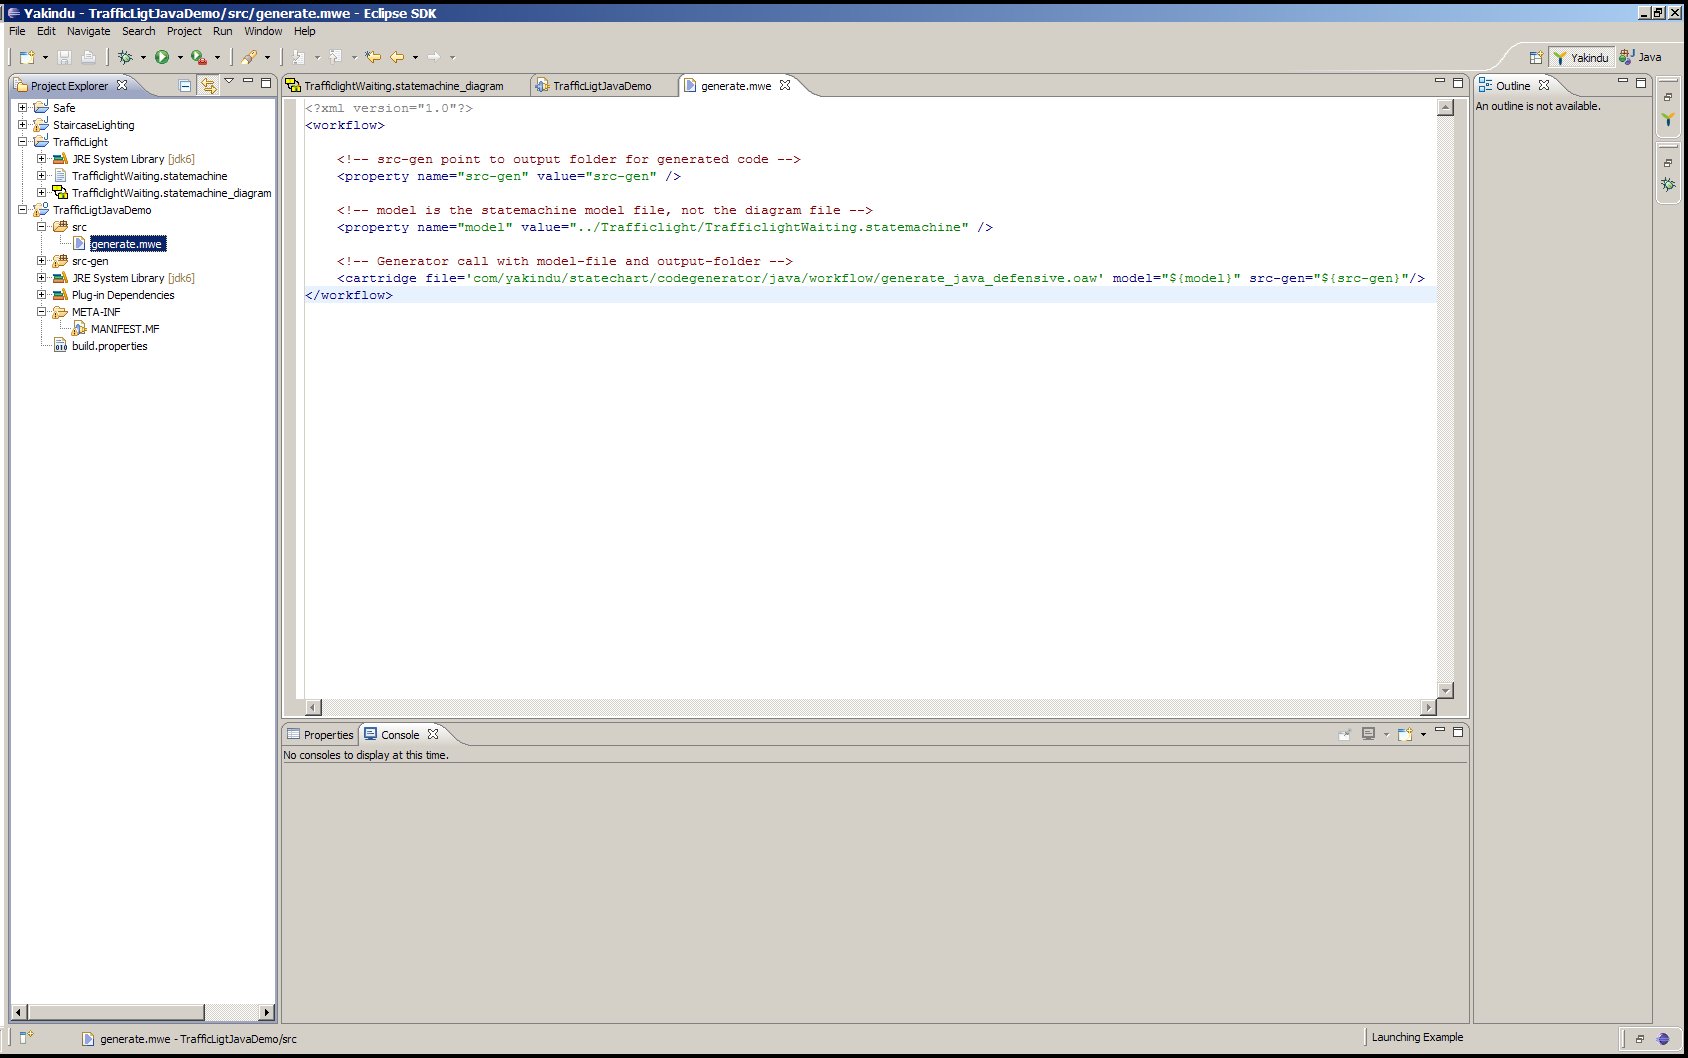
\includegraphics[width=\textwidth]{./Pictures/Screenshot13}
\caption{\label{fig:screenshot13}}
\end{figure}

In fact, the YAKINDU Statechart Java Codegenerator provides a lot of workflow
cartridges, namely \emph{generate\_java.oaw}, \emph{generate\_java\_me.oaw} and
\emph{generate\_java\_lejos.oaw}. Each has a defensive-version, which
basically generate the same sort of
Java source code, with the restriction that the \emph{defensive} version
generates additional defensive code, being used to check pre- and
post-conditions as well as invariants at runtime.
The Java-Codegenerator generates normal JavaSE-Code. The JavaME-Code is designed
for mobile devices, which doesn't supports all Javaclasses.
The third workflow cartridge generate Java-Code for leJOS, which can deploy on a
LEGO Mindstorm.

\clearpage
\subsection{Execute MWE Workflow}
Having specified all relevant workflow properties, and having specified to
call the code generator cartridge, the MWE workflow may then be simply
executed as depicted by Figure \ref{fig:screenshot14}. It will generate Java
source code into the selected folder (here, the local \texttt{src-gen} folder
within the \emph{TrafficLightJavaDemo} project).

\begin{figure}[h!]
\center
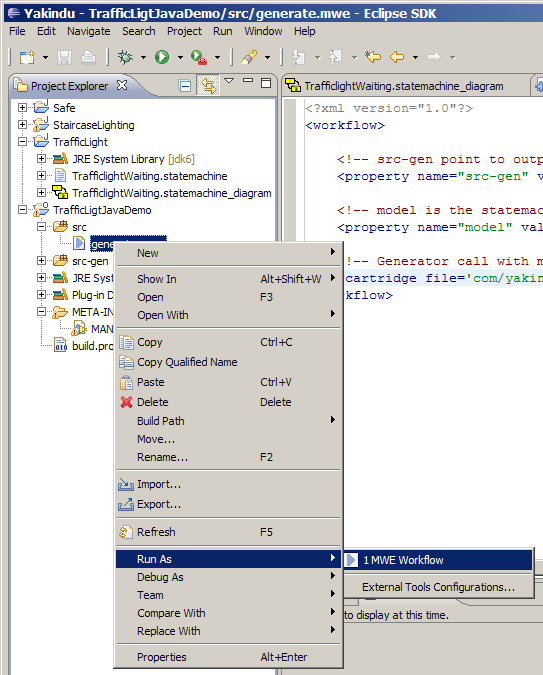
\includegraphics[width=0.5\textwidth]{./Pictures/Screenshot14}
\caption{\label{fig:screenshot14} Contents of MWE Workflow File}
\end{figure}

\clearpage